\section{Use Cases}
\label{s:usecases}


We developed two benchmark applications after discussions with environmental
scientists, astronomists, and geneticists.  The first is an image processing
benchmark developed with scientists at the Large Synoptic Survey Telescope
(LSST) project.  It is very similar to environmental science requirements, so
they are combined together. The second was developed with geneticists at the
Broad Institute\footnote{\url{http://www.broadinstitute.org/}}.  Each benchmark
consists of a workflow description, a dataset, and lineage queries.  We used
the benchmarks to design the optimizations described in the paper.   This
section will briefly describe each benchmark's scientific application, the
types of desired lineage queries, and application-specific insights.


\subsection{Astronomy} 
\label{s:ucastro}



The Large Synaptic Survey Telescope (LSST) is a wide angle telescope slated to
begin operation in Fall 2015.  A key challenge in processing telescope images is
filtering out high energy particles (cosmic rays) that create abnormally bright
pixels in the resulting image, which can be mistaken for stars.  The telescope
compensates  by taking two consecutive pictures of the same piece of the sky
and removing the cosmic rays in software.  The LSST image processing workflow
(Figure \ref{f:lsstworkflow}) takes two images as input and outputs an
annotated image that labels each pixel with the celestial body it belongs to.
It first cleans and detects cosmic rays in each image separately, then creates
a single composite, cosmic-ray-free, image that is used to detect celestial
bodies.  There are 22 SciDB built-in operators (blue solid boxes) that perform
common matrix operations, such as convolution, and four UDFs (red dotted boxes
labeled A-D).  The UDFs A and B output cosmic-ray masks for each of the images.
After the images are subsequently merged, C removes cosmic-rays from the
composite image, and D detects stars from the cleaned image.  


The LSST scientists are interested in three types of queries.  The first picks
a star in the output image and traces the lineage back to the initial
input image to detect bad input pixels.  The latter two queries select a
region of output (or input) pixels and trace the pixels backward (or forward)
through a subset of the workflow to identify a single faulty operator.  
%These queries only partially trace through the workflow because it is often a
%single operator that is the obvious point of error.  
As an example, suppose the operator that computes the mean brightness of the
image  generated an anomalously high value due to a few bad pixel, which led to
further mis-calculations.  The astronomer might work backward from those
calculations, identify the input pixels that contributed to them, and filter out
those pixels that appear excessively bright.

Both the LSST and environmental scientists described workloads where the majority
of the data processing code computes output pixels using input pixels within a
small distance from the corresponding coordinate of the output pixel.  These
regions may be constant, pre-defined values, or easily computed from a small
amount of additional metadata.  For example, a pixel in the mask produced by
cosmic ray detection ($CRD$) is set if the related input pixel is a cosmic ray,
and depends on neighboring input cells within 3 pixels.  Otherwise, it only
depends on the related input pixel.  They also felt that it is sufficient for lineage queries
to return a superset of the exact lineage.  Although we do not take
advantage of this insight, this suggests future work in lossy compression
techniques.




\begin{figure}[h] \centerline{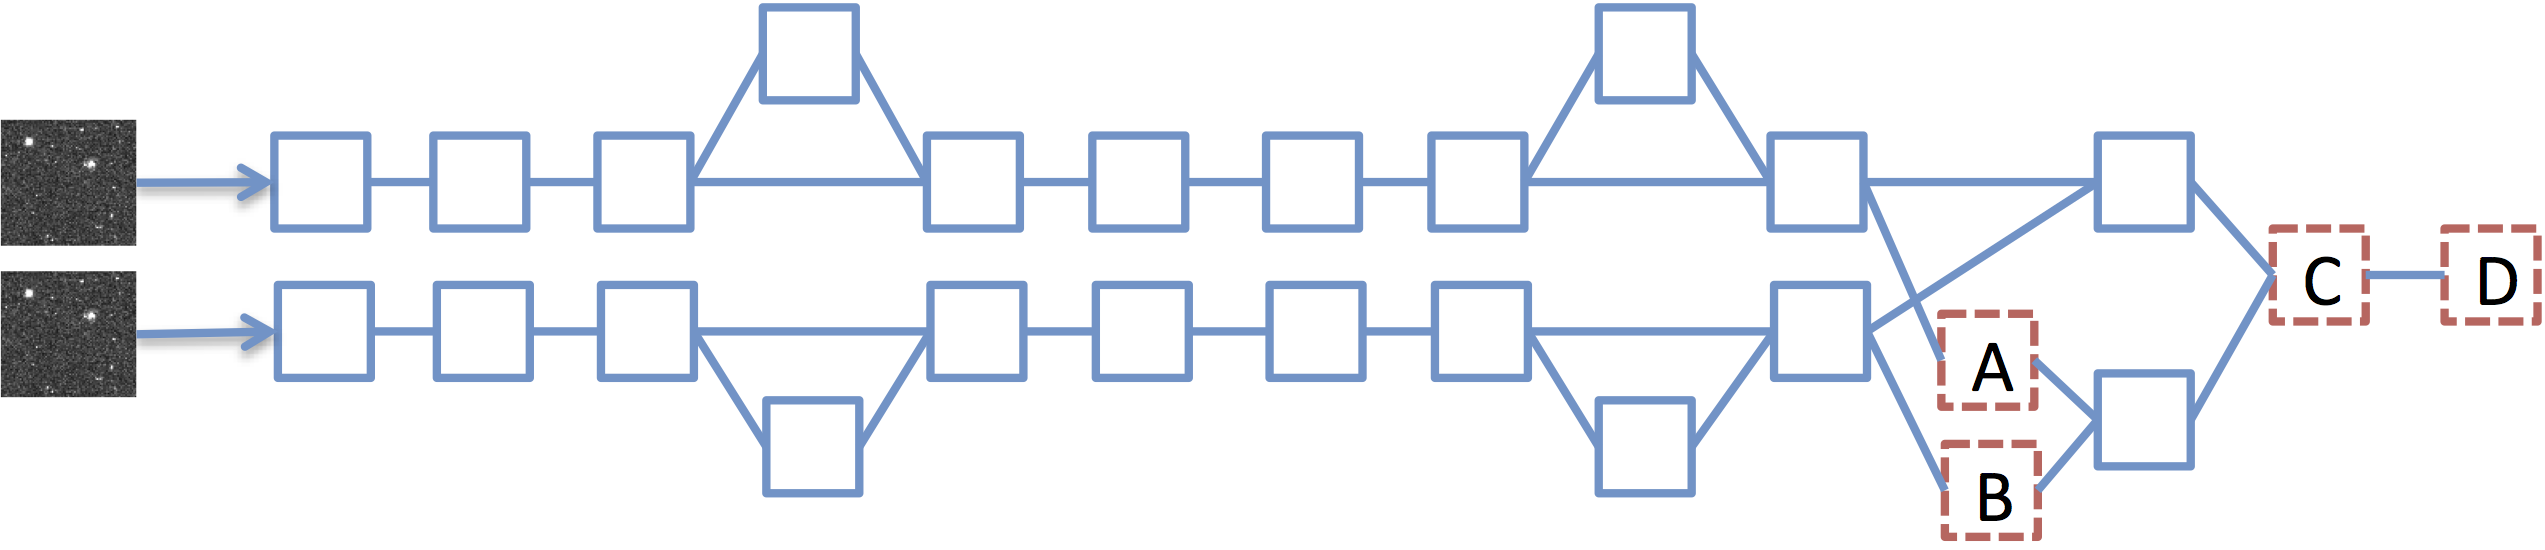
\includegraphics[width=3.3in,natwidth=8.49in,natheight=1.84in]{figures/lsst.png}}
\caption{Summary diagram of LSST workflow.  Each solid rectangle is a SciDB
native operator while the red dotted rectangles are UDFs.}
\label{f:lsstworkflow} \end{figure}
 













\subsection{Genomics Prediction} \label{s:ucgenomics}


We have also been working with researchers at the Broad Institute on a genomics
benchmark related to predicting recurrences of medulloblastoma in patients.
Medulloblastoma is a form of cancer that spawns brain tumors that spread
through the cerebrospinal fluid.  Pablo et.~al~\cite{pablo} have identified a
set of patient features that help predict relapse in medulloblastoma patients
that have been treated.  The features include histology, gene expression levels,  and the existence of genetic abnormalities.  The
workflow (Figure \ref{f:genomicsworkflow}) is a two-step process that first
takes a training patient-feature matrix and outputs a Bayesian model.  Then it
uses the model to predict relapse in a test patient-feature matrix.  The model
computes how much each feature value contributes to the likelihood of patient
relapse.  The ten built-in operators (solid blue boxes) are simple matrix
transformations.  The remaining UDFs extract a subset of the input arrays
(E,G), compute the model (F), and predict the relapse probability (H).

The model is designed to be used by clinicians through a visualization that
generates lineage queries.  The first query picks a relapse prediction and traces its
lineage back to the training matrix to find supporting input data. The second
query picks a feature  from the model and traces it back to the training
matrix to find the contributing input values.  The third query points at a set
of training values and traces them forward to the model, while the last query
traces them to the end of the workflow to find the predictions they affected.

The genomics benchmark can devote up-front storage and runtime overhead to
ensure fast  query execution because it is an interactive visualization.
Although this is application specific, it suggests that scientific applications
have a wide range of storage and runtime overhead constraints.



\begin{figure}[h] \centerline{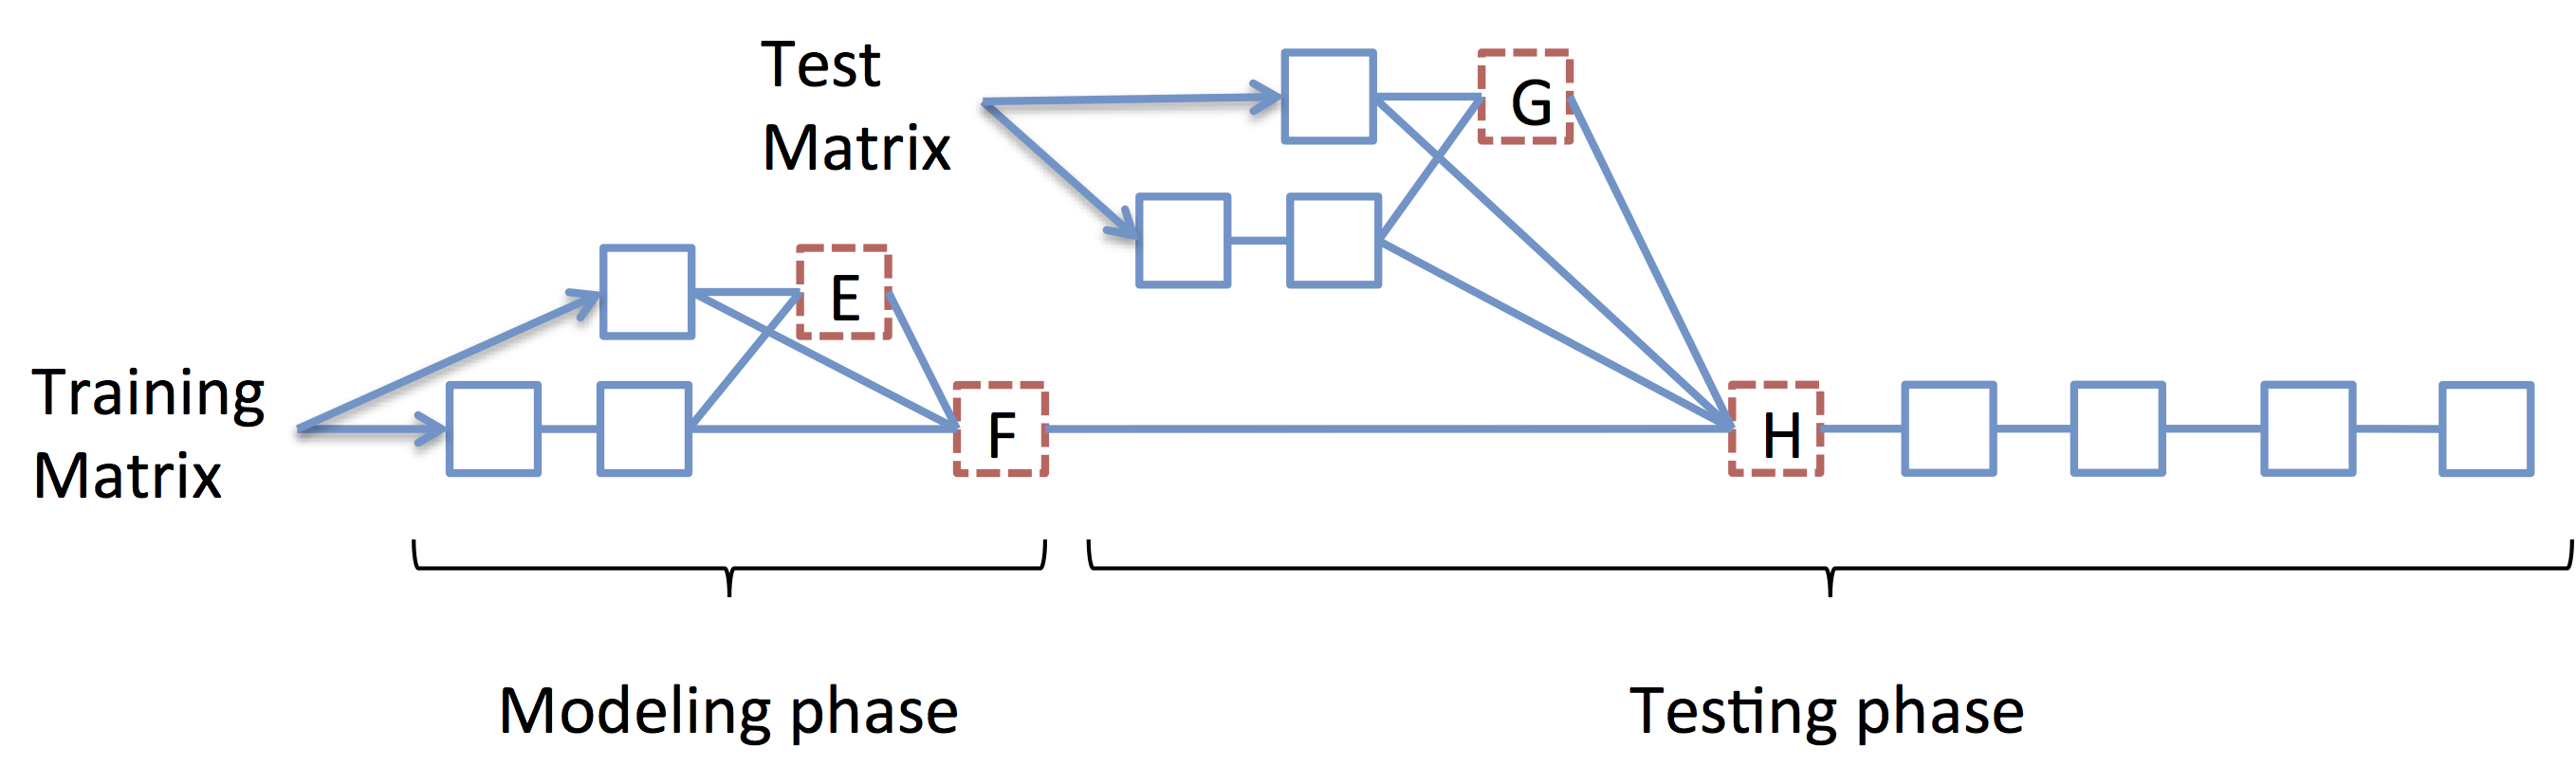
\includegraphics[width=3.3in,natwidth=9.06in,natheight=2.7in]{figures/genomics.png}}
\caption{Simplified diagram of genomics workflow.  Each solid rectangle is a
SciDB native operator while the red dotted rectangles are UDFs.}
\label{f:genomicsworkflow} \end{figure}



